\documentclass{article}
\usepackage[utf8]{inputenc}

% Page setup
\usepackage[a4paper,landscape,margin=2cm]{geometry}
\usepackage{amsmath}

% Typography
\usepackage[scaled]{helvet}
\let\familydefault\sfdefault

\usepackage[usenames,svgnames]{xcolor}
\usepackage{tikz,pgfplots}
\usetikzlibrary{positioning,arrows,intersections,calc}

\definecolor{colorwhite}    {RGB}{255,255,255}
\definecolor{colorpod}      {RGB}{199,212,104}
\definecolor{colorbook}     {RGB}{ 79,142,209}
\definecolor{colorprofile}  {RGB}{143,232,186}
\definecolor{colortext}     {RGB}{ 29, 29, 27}
\definecolor{colorkey}      {RGB}{129, 29, 27}
\definecolor{colorperson}   {RGB}{190, 22, 34}

\begin{document}
\pagestyle{empty}
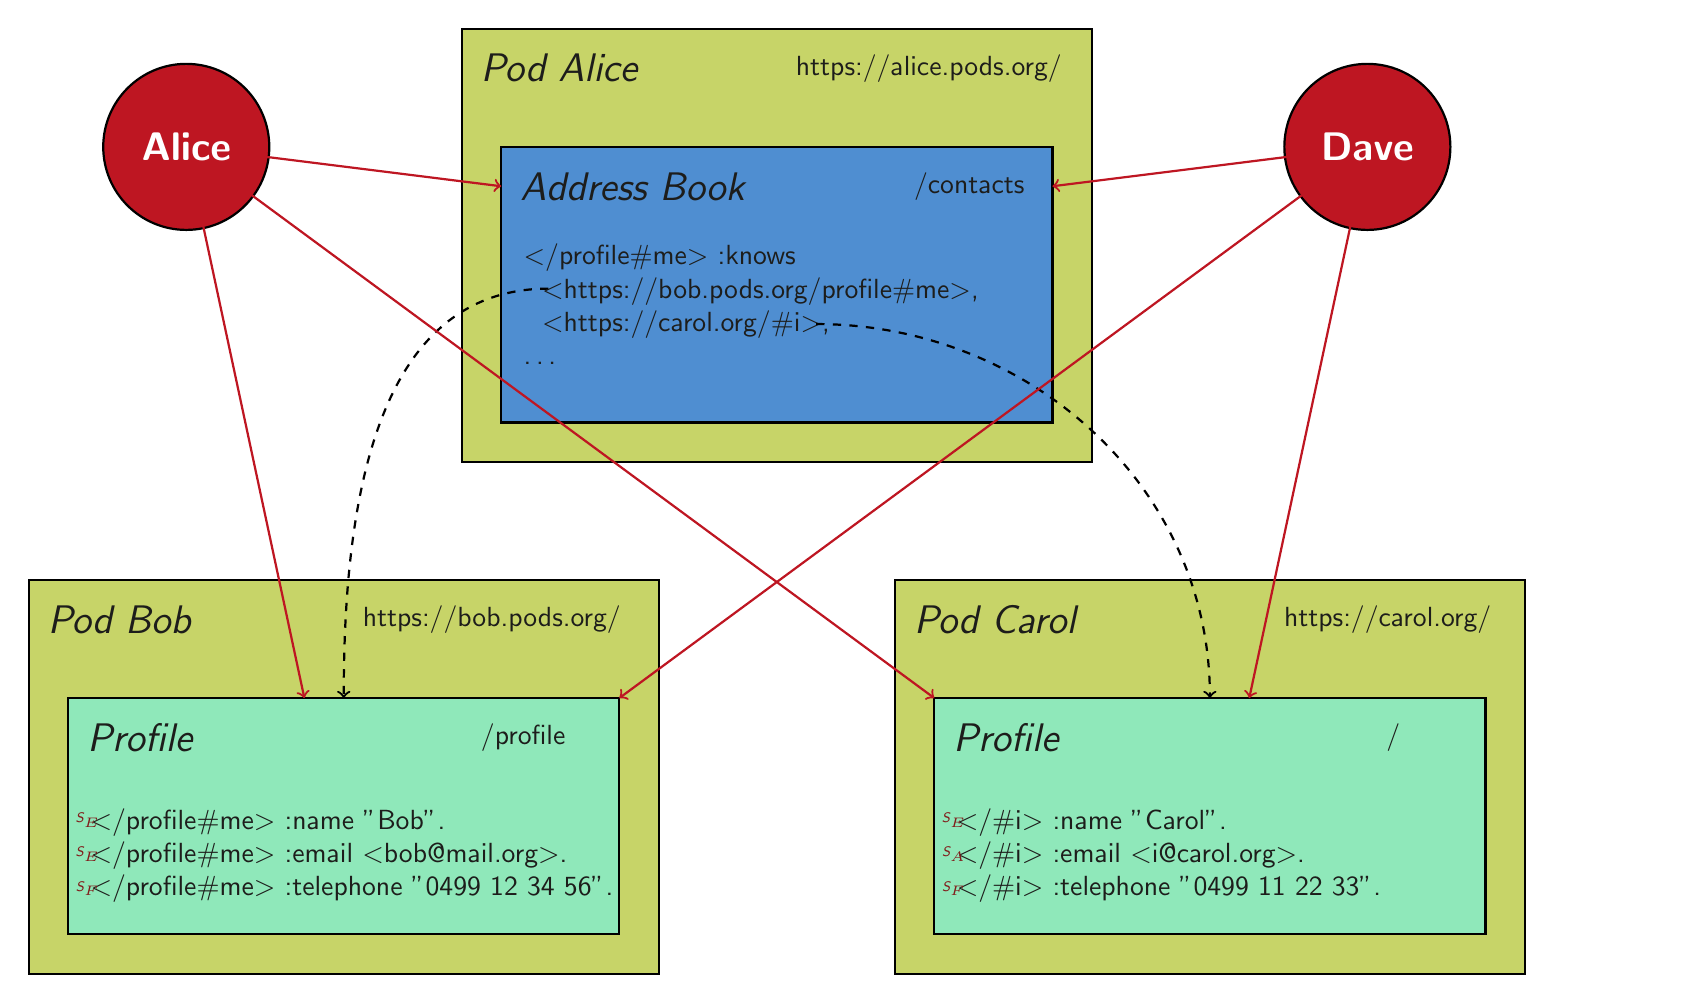
\begin{tikzpicture}[
    node distance = 10em, auto, thick,
    title/.style={text=colortext,font={\Large\itshape}},
    person/.style={text=colorwhite,font={\Large\bfseries}},
    code/.style={text=colortext,font={}},
    key/.style={text=colorkey,font={\tiny\itshape}}
]

    % Person Alice
    \draw[fill=colorperson] (2,4) circle (30pt);
    \node[person] at (2,4) (alice) {Alice};

    % Person Dave
    \draw[fill=colorperson] (17,4) circle (30pt);
    \node[person] at (17,4) (dave) {Dave};

    % Pod Alice
    \draw[fill=colorpod] (5.5,0) rectangle (13.5,5.5);
    \node[title,text width=10em] at (7.5,5) {Pod Alice};
    \node[code,text width=10em] at (11.5,5) {https://alice.pods.org/};

    % Address Book Alice
    \draw[fill=colorbook] (6,0.5) rectangle (13,4);
    \node[title,text width=10em] at (8,3.5) {Address Book};
    \node[code,text width=10em] at (13,3.5) {/contacts};
    \node[code,text width=20em] at (9.8,2) {$<$/profile\#me$>$ :knows\\
    \ \ $<$https://bob.pods.org/profile\#me$>$,\\
    \ \ $<$https://carol.org/\#i$>$,\\
    \ldots};

    % Pod Bob
    \draw[fill=colorpod] (0,-6.5) rectangle (8,-1.5);
    \node[title,text width=10em] at (2,-2) {Pod Bob};
    \node[code,text width=10em] at (6,-2) {https://bob.pods.org/};

    % Profile Bob
    \draw[fill=colorprofile] (0.5,-6) rectangle (7.5,-3);
    \node[title,text width=10em] at (2.5,-3.5) {Profile};
    \node[code,text width=10em] at (7.5,-3.5) {/profile};
    \node[code,text width=20em] at (4.3,-5) {$<$/profile\#me$>$ :name "Bob".\\
    $<$/profile\#me$>$ :email $<$bob@mail.org$>$.\\
    $<$/profile\#me$>$ :telephone "0499 12 34 56".};
    \node[key] at (0.75,-4.55) {S$_E$};
    \node[key] at (0.75,-4.98) {S$_E$};
    \node[key] at (0.75,-5.42) {S$_F$};
    %\node[key] at (4,-6.25) {Alice $\in$ S$_F$; Dave $\in$ S$_E$};

    % Pod Carol
    \draw[fill=colorpod] (11,-6.5) rectangle (19,-1.5);
    \node[title,text width=10em] at (13,-2) {Pod Carol};
    \node[code,text width=10em] at (17.7,-2) {https://carol.org/};

    % Profile Carol
    \draw[fill=colorprofile] (11.5,-6) rectangle (18.5,-3);
    \node[title,text width=10em] at (13.5,-3.5) {Profile};
    \node[code,text width=10em] at (19,-3.5) {/};
    \node[code,text width=20em] at (15.3,-5) {$<$/\#i$>$ :name "Carol".\\
    $<$/\#i$>$ :email $<$i@carol.org$>$.\\
    $<$/\#i$>$ :telephone "0499 11 22 33".};
    \node[key] at (11.75,-4.55) {S$_E$};
    \node[key] at (11.75,-4.98) {S$_A$};
    \node[key] at (11.75,-5.42) {S$_F$};
   % \node[key] at (15,-6.25) {Alice $\in$ S$_A$; Dave $\in$ S$_E$};

    % Arrows between pods
    \draw[->,thick,dashed](6.6,2.2) to [out=180,in=90] (4,-3);
    \draw[->,thick,dashed](10,1.75) to [out=0,in=90] (15,-3);

    % Arrows from people to data
    \draw[->,thick,colorperson] (alice) -- (6,3.5);
    \draw[->,thick,colorperson] (alice) -- (3.5,-3);
    \draw[->,thick,colorperson] (alice) -- (11.5,-3);
    \draw[->,thick,colorperson] (dave)  -- (13,3.5);
    \draw[->,thick,colorperson] (dave)  -- (7.5,-3);
    \draw[->,thick,colorperson] (dave)  -- (15.5,-3);

\end{tikzpicture}
\end{document}
